\documentclass{standalone}
\usepackage{tikz}
\usetikzlibrary{calc}

\begin{document}

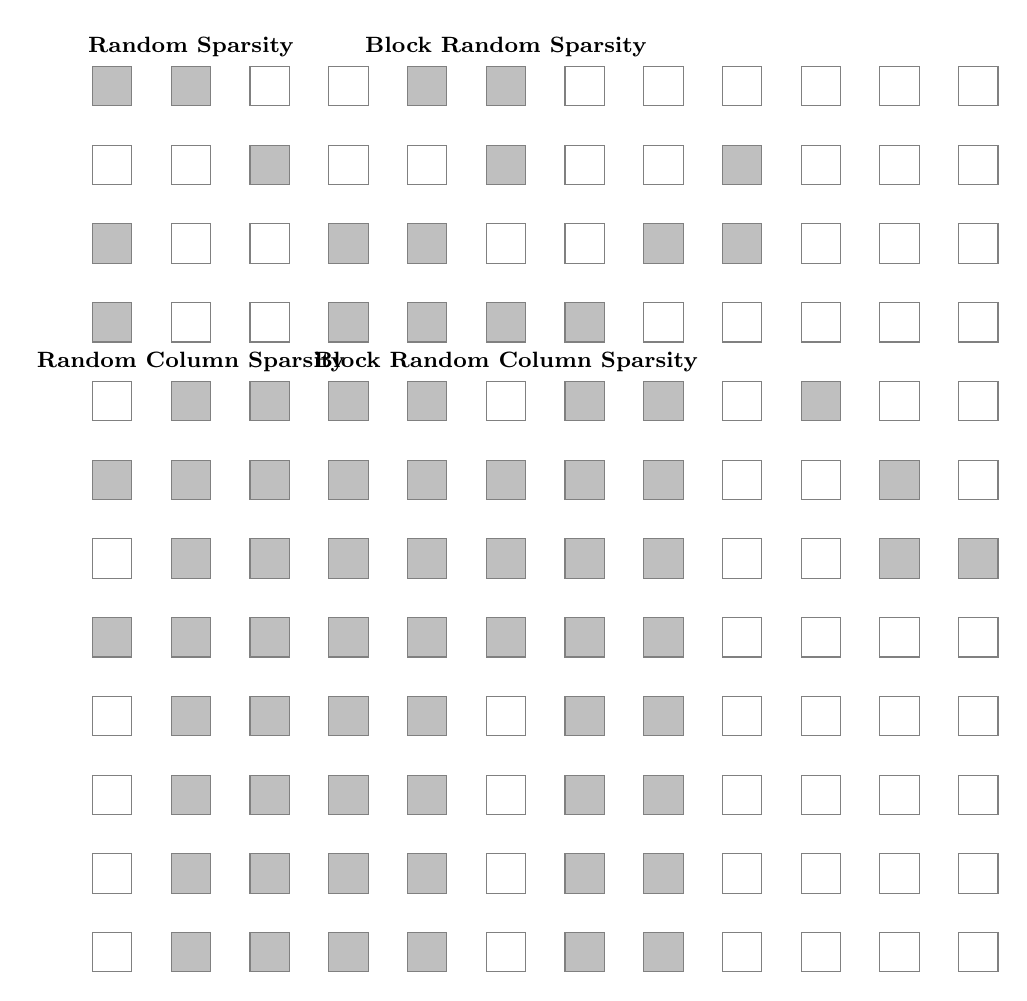
\begin{tikzpicture}[
    cell/.style={rectangle, draw=gray, minimum size=0.5cm},
    caption/.style={below, node distance=1pt, font=\footnotesize}]

    % Define the grid size
    \def\gridSize{8}
    
    % Captions for each sparsity type
    \node[font=\footnotesize\bfseries] at (2, 8.5) {Random Sparsity};
    \node[font=\footnotesize\bfseries] at (6, 8.5) {Block Random Sparsity};
    \node[font=\footnotesize\bfseries] at (2, 4.5) {Random Column Sparsity};
    \node[font=\footnotesize\bfseries] at (6, 4.5) {Block Random Column Sparsity};

    % Random Sparsity
    \foreach \x in {1,...,8} {
        \foreach \y in {1,...,8} {
            \pgfmathrandominteger{\a}{1}{100}
            \ifnum\a > 50
                \node[cell, fill=gray!50] at (\x, \y) {};
            \else
                \node[cell] at (\x, \y) {};
            \fi
        }
    }

    % Block Random Sparsity
    \foreach \x in {1,...,8} {
        \pgfmathrandominteger{\blockStart}{1}{6}
        \pgfmathrandominteger{\blockLength}{2}{3}
        \foreach \y in {1,...,8} {
            \ifnum\y > \blockStart \relax
            \ifnum\y < \number\numexpr\blockStart+\blockLength\relax
                \node[cell, fill=gray!50] at (\x+4, \y) {};
            \else
                \node[cell] at (\x+4, \y) {};
            \fi
            \else
                \node[cell] at (\x+4, \y) {};
            \fi
        }
    }

    % Random Column Sparsity
    \foreach \x in {1,...,8} {
        \pgfmathrandominteger{\a}{1}{100}
        \ifnum\a > 50
            \foreach \y in {1,...,8} {
                \node[cell, fill=gray!50] at (\x, \y-4) {};
            }
        \else
            \foreach \y in {1,...,8} {
                \node[cell] at (\x, \y-4) {};
            }
        \fi
    }

    % Block Random Column Sparsity
    \pgfmathrandominteger{\blockColStart}{1}{6}
    \pgfmathrandominteger{\blockColLength}{2}{3}
    \foreach \x in {1,...,8} {
        \ifnum\x > \blockColStart \relax
        \ifnum\x < \number\numexpr\blockColStart+\blockColLength\relax
            \foreach \y in {1,...,8} {
                \node[cell, fill=gray!50] at (\x+4, \y-4) {};
            }
        \else
            \foreach \y in {1,...,8} {
                \node[cell] at (\x+4, \y-4) {};
            }
        \fi
        \else
            \foreach \y in {1,...,8} {
                \node[cell] at (\x+4, \y-4) {};
            }
        \fi
    }
\end{tikzpicture}

\end{document}